\section{Session 3. Unconstrained optimization}

Let $f$ be a function of $n$ variables and let $1 \leq i \leq n$ and $1 \leq j \leq n$. If the partial derivatives $f'_i$ and $f'_j$ of $f$ exist in an open set $S$ containing $(x_1,\ldots, x_n)$ and both of these partial derivatives are differentiable at $(x_1, \ldots, x_n)$ then $(\Hessian f)_{ij}=(\Hessian f)_{ji}$.

\begin{itemize}
  \item If the Hessian at a given point has all positive eigenvalues, it is said to be a positive-definite matrix. This is the multivariable equivalent of “concave up” (we called it "convex" in this course).
  \item If all of the eigenvalues are negative, it is said to be a negative-definite matrix. This is like “concave down”. (we call it "concave" in this course).
  \item If either eigenvalue is 0, then you will need more
  information (possibly a graph or table) to see what
  is going on.
  \item It the eigenvalues are mixed, you have a saddle point.
\end{itemize}

\begin{Exercise}
  Determine the concavity of
\[f(x, y) = x^3 + 2y^3 - xy\]
at the following points:
\begin{enumerate}
  \item (0, 0)
  \item (3, 3)
  \item (3, -3)
  \item (-3, 3)
  \item (-3, -3)
\end{enumerate}
\end{Exercise}
%------------------------------------------------%------------------------------------------------
\begin{Exercise}
  Study the critical points of the functions 
  \begin{enumerate}
    \item $f(x,y)=4x+2y-x^2-3y^2$
    \item $f(x, y) = x^4 + y^2 - xy$
  \end{enumerate}
  
\end{Exercise}


\begin{Exercise}
    Check the character of the stationary point in $(0,0)$ for the functions:
    \begin{enumerate}
      \item $f(x,y)=x^2+y^2$
      \item $g(x,y)=-x^2-y^2$
      \item $h(x,y)=x^2-y^2$
      \item $k(x,y)=x^3+2y^3-xy$ (is it concave or convex in $(3,3)$? what about in $(-3,-3)$?)
    \end{enumerate}

\end{Exercise}

%------------------------------------------------%------------------------------------------------
  \begin{center}
    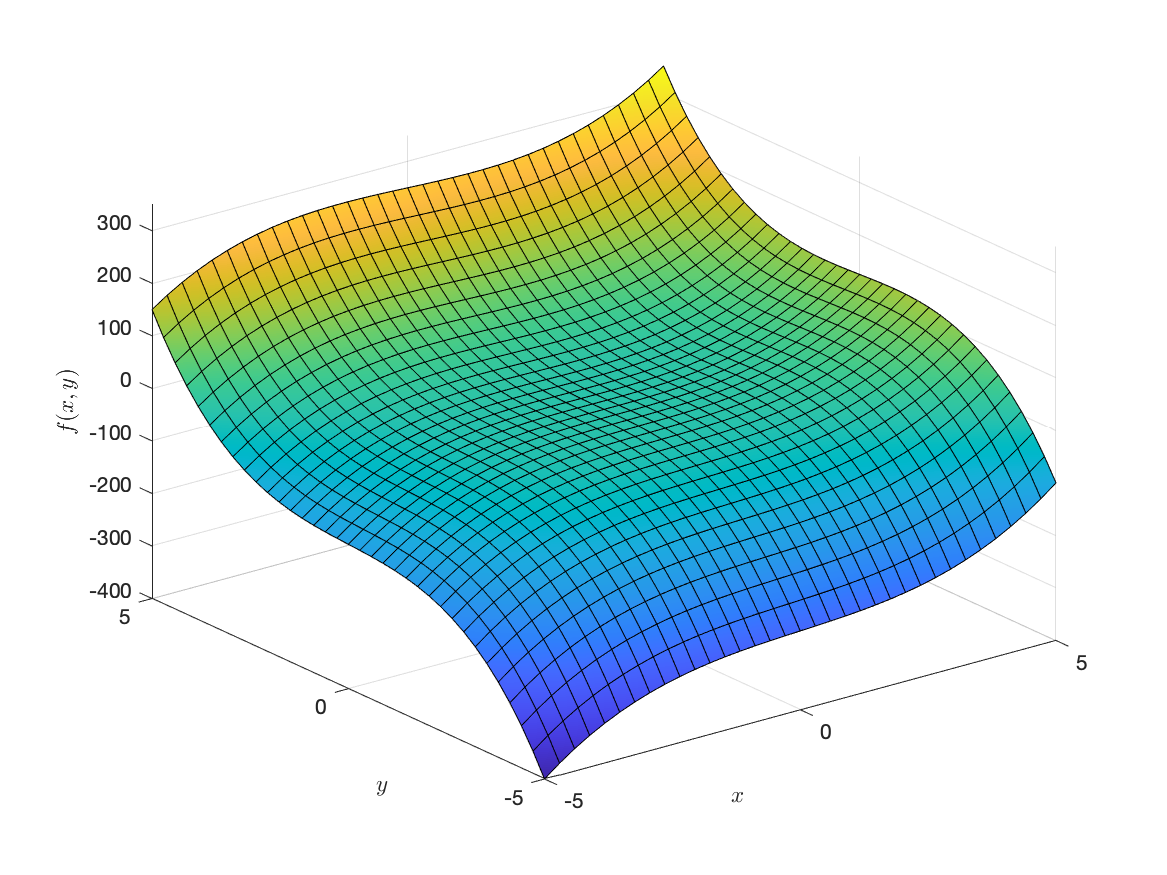
\includegraphics[width=0.8\textwidth]{../figures/x3plus2y3minusxy.png}
  \end{center}

%------------------------------------------------%------------------------------------------------
  For unconstrained problems with just one variable $x$, if first and second derivatives exist in $x^*$:
  \begin{description}
    \item[Necessary conditions] If $\frac{df}{dx}=0$ at $x=x^*$
    \begin{itemize}
      \item $\frac{d^2f}{dx^2}\geq 0$, for a local minimum at $x=x^*$
      \item $\frac{d^2f}{dx^2}\leq 0$, for a local maximum at $x=x^*$
    \end{itemize}
    \item[Sufficient conditions] If $\frac{df}{dx}=0$ at $x=x^*$
    \begin{itemize}
      \item $\frac{d^2f}{dx^2}> 0$, for a local minimum at $x=x^*$
      \item $\frac{d^2f}{dx^2}< 0$, for a local maximum at $x=x^*$
    \end{itemize}
  \end{description}
%------------------------------------------------%------------------------------------------------
  For unconstrained problems with several variables $\uvec{x}=(x_1,\ldots,x_n)$:
  \begin{description}
    \item[Sufficient condition] If $\pdv{f}{x_i}=0$ at $\uvec{x}=\uvec{x}^*$:
    \begin{itemize}
      \item $\grad{f}=\uvec{0}$, for a local minimum at $x=x^*$ if the function is convex;
      \item $\grad{f}=\uvec{0}$, for a local maximum at $x=x^*$ if the function is concave.
    \end{itemize}
    \item[Decision conditions] The function $f$ is a convex function if $H_f$ is positive definite or positive semidefinite for all $\uvec{x}$; and $f$ is concave if $H_f$ is negative definite or negative semidefinite for all $\uvec{x}$. For $f:\mathbf{R}^2\rightarrow\mathbf{R}$
    \[
      {\mathbf H}_f(x,y)=\begin{pmatrix} \frac{\partial^2 f}{\partial x^2} & \frac{\partial^2 f}{\partial x \partial y} \\ \frac{\partial^2 f}{\partial y \partial x} & \frac{\partial^2 f}{\partial y^2}\end{pmatrix} =
      \begin{pmatrix} A & C \\ C & B \end{pmatrix}
\]
  \end{description}

  Let $f$ be a twice-differentiable function of many variables on the convex open set $S$ and denote the Hessian of $f$ at the point $x$ by $H(x)$. Then
\begin{itemize}
  \item $f$ is concave if and only if $H(x)$ is negative semidefinite $\forall x \in S$
  \item if $H(x)$ is negative definite $\forall x \in S$ then $f$ is strictly concave (see Eq. \ref{eq:convex})
  \item $f$ is convex if and only if $H(x)$ is positive semidefinite $\forall x \in S$
  \item if $H(x)$ is positive definite $\forall x \in S$ then $f$ is strictly convex (see Eq. \ref{eq:convex})
\end{itemize}

%------------------------------------------------%------------------------------------------------
  Things are not so simple if, for example, functions are not derivable in $x^*$:
  \begin{center}
    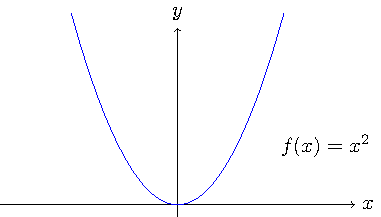
\includegraphics[width=0.4\textwidth]{x2.pdf}
    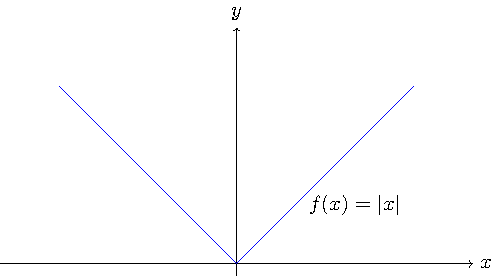
\includegraphics[width=0.4\textwidth]{absx.pdf}
  \end{center}
  Or, if the function is not convex (nor concave), the sufficient condition is lost and we may find local optimal points, instead of global.

  For constrained optimization problems, the shape of the feasible region adds difficulty.



%------------------------------------------------%------------------------------------------------
\subsection{Iterative methods}

\subsubsection{Line search}
Let us assume a concave function. First, establish error tolerance $\epsilon$. Then:
  \begin{enumerate}
    \item Set up lower and upper bounds for $x$ by finding $x_l,x_u$ such that $\frac{df}{dx_l}\geq 0$ and $\frac{df}{dx_u}\leq 0$
    \item Get new trial intermediate solution (eg, $x=\frac{x_l+x_u}{2}$)
    \item If $x_u-x_l\leq \epsilon$, then terminate
    \item If $\frac{df}{dx}\geq 0$, set $x_l=x$; if $\frac{df}{dx}\leq 0$, set $x_u=x$
    \item Go to step 1
  \end{enumerate}

  For an implementation, see \href{https://machinelearningmastery.com/line-search-optimization-with-python/}{this link}
%------------------------------------------------%------------------------------------------------
For a continuous function it guarantees to find an extremum.

\subsubsection{Golden search}
   Two quantities are in the golden ratio if their ratio is the same as the ratio of their sum to the larger of the two quantities:
\[
\frac{a+b}{a}=\frac{a}{b}=\psi \Rightarrow \psi=\frac{1+\sqrt{5}}{2}=1.616033988...
\]


Procedure of the Golden search method, given a function  to be minimized, $f(x)$, the interval to be searched as $x\in(x_1,x_4)$, and their functional values $f(x_1)$ and $f(x_2)$:
\begin{enumerate}
  \item Calculate an interior point and its functional value $f(x_3$). Ensure the position of $x_3$ follows the golden ratio between the distances $\frac{x_2-x_1}{x_3-x_1}=\frac{x_3-x_1}{x_2-x_3}=\psi$.
  \item Using the triplet, determine if convergence criteria are fulfilled. If they are, estimate the $x$ at the minimum from that triplet and terminate/return.
  \item Select $x_4$ within the largest interval, following the same ratios as in Step 1.
  \item The three points for the next iteration will be the one where $f(x)$ is a minimum, and the two points closest to it in $x$.
  \item Go to step 2.
\end{enumerate}

\begin{Exercise}
  Use the Golden Search method to find the minimum of function $f(x)=x^2-6x+15$ in the interval $x\in(0,10)$. Set up a spreadsheet to do so.
  %https://www.youtube.com/watch?v=hLm8xfwWYPw
\end{Exercise}


%------------------------------------------------%------------------------------------------------
\begin{program}
  E2. Build a Python code that can run one-dimensional search algorithms for user defined functions, using or not first derivatives. Implement the one-dimensional line search and the golden search algorithms and find the optimal solution for the functions:
  \begin{itemize}
    \item $f(x)=x^4-16x^3+45 x^2-20x+203$ within the range $x\in(2.5,14)$
    \item $g(x)=x^5-2x^4-23x^3-12x^2+36x$ within the range $x\in(2,3)$
  \end{itemize}
  Try both a direct implementation as well as the use of solvers in scipy.
\end{program}

\begin{Exercise}
  Draw the {\em Rosenbruck's function}, $f(x,y)=100(y-x^2)^2+(1-x)^2$ and discuss on its convexity, the feasibility of its minimization and the most appropriate numerical method to use.
\end{Exercise}


%------------------------------------------------%------------------------------------------------

%https://suzyahyah.github.io/calculus/optimization/2018/04/06/Taylor-Series-Newtons-Method.html
  As a reference (not the central aim of this course) here is a list of some algorithms/methods to explore to perform unconstrained optimization in multiple dimensions:
  \begin{itemize}
    \item Newton's method,
    \item Quasi-Newton methods (e.g., \href{https://machinelearningmastery.com/bfgs-optimization-in-python/}{BFGS}),
    \item Trust-region methods,
    \item \href{https://en.wikipedia.org/wiki/Conjugate_gradient_method}{Conjugated gradient methods}.
  \end{itemize}
  and their many variants.

